\documentclass[11pt,a4paper]{article}
\usepackage[utf8]{vietnam}
\usepackage{amsmath,amssymb}
\usepackage{geometry}
\geometry{top=1.5cm,bottom=1.2cm,left=1.4cm,right=1.4cm,headheight=28pt,headsep=12pt,footskip=18pt}
\usepackage{tikz}
\usepackage{xcolor}
\usepackage{graphicx}
\usepackage{fancyhdr}
\usepackage{tabularx}
\usepackage{enumitem}

\renewcommand{\baselinestretch}{1.08}
\setlength{\parskip}{2pt}
\setlength{\parindent}{0pt}

\definecolor{hfRed}{RGB}{211,47,47}
\definecolor{hfGreen}{RGB}{139,195,144}
\definecolor{myGreen}{RGB}{46,125,50}
\definecolor{myBlue}{RGB}{21,101,192}
\definecolor{mySub}{RGB}{0,105,92}
\definecolor{myPurple}{RGB}{106,27,154}

\pagestyle{fancy}
\fancyhf{}
\fancyhead[L]{\small\itshape\color{hfRed} Tài liệu lưu hành nội bộ}
\fancyhead[R]{\small\itshape\color{hfRed} Thầy \textbf{TRẦN VĂN THẠNH} - 0777.470.803}
\renewcommand{\headrulewidth}{0.8pt}
\renewcommand{\headrule}{\hbox to\headwidth{\color{hfGreen}\leaders\hrule height \headrulewidth\hfill}}

\fancyfoot[L]{\small\itshape\color{hfRed} CS1: 6/15 Nguyễn Hoàng, P. Kim Long, TP Huế \quad|\quad CS2: 24 Đặng Thái Thân, TP Huế}
\fancyfoot[R]{\small\bfseries\color{hfRed} Trang \thepage}
\renewcommand{\footrulewidth}{0.8pt}
\renewcommand{\footrule}{\hbox to\headwidth{\color{hfGreen}\leaders\hrule height \footrulewidth\hfill}}

\begin{document}

% --- HEADER BLOCK ---
\begin{tabularx}{\textwidth}{@{}l X r@{}}
\textbf{\small SỞ GIÁO DỤC VÀ ĐÀO TẠO} & & \textbf{\small ĐỀ KIỂM TRA GIỮA HỌC KÌ I} \\
\textbf{\normalsize TRƯỜNG THPT CHUYÊN / THPT} & & \textbf{\normalsize MÔN: HÓA HỌC - LỚP 10} \\
\textit{\small (Đề thi gồm có 03 trang)} & & \textit{\small Thời gian làm bài: 45 phút (không kể phát đề)}
\end{tabularx}

\begin{center}

\textbf{Họ và tên thí sinh:} \dotfill \quad \textbf{Lớp:} \dots\dots\dots \quad \textbf{Số báo danh:} \dots\dots\dots \hfill \textbf{\large Mã đề 101}
\end{center}
\vspace{-4pt}
{\color{gray!50}\hrule height 0.8pt}
\vspace{6pt}

% =============================================================================
% PHẦN I
% =============================================================================
{\color{myGreen}\bfseries\large PHẦN I (3,0 ĐIỂM). Câu trắc nghiệm nhiều phương án lựa chọn.}

\textit{\small Thí sinh trả lời từ câu 1 đến câu 12. Mỗi câu hỏi thí sinh chỉ chọn một phương án.}
\vspace{3pt}

% CÂU 1
\textbf{Câu 1.} Phát biểu nào sau đây \textbf{không đúng}?
\begin{enumerate}[label=\textbf{\Alph*.},leftmargin=*,itemsep=1pt,topsep=1pt]
\item Số khối của hạt nhân bằng tổng số proton và số neutron.
\item Nguyên tố hoá học là những nguyên tử có cùng số đơn vị điện tích hạt nhân.
\item Số hiệu nguyên tử bằng số đơn vị điện tích hạt nhân nguyên tử.
\item Trong nguyên tử, số đơn vị điện tích hạt nhân bằng số proton và bằng số neutron.
\end{enumerate}


% CÂU 2
\textbf{Câu 2.} Nguyên tử chứa những hạt mang điện là
\begin{enumerate}[label=\textbf{\Alph*.},leftmargin=*,itemsep=1pt,topsep=1pt]
\item proton và electron.
\item proton và $\alpha$.
\item electron và neutron.
\item proton và neutron.
\end{enumerate}


% CÂU 3
\textbf{Câu 3.} Sự phân bố electron theo orbital nào dưới đây là đúng?
\begin{center}
\begin{tabularx}{\textwidth}{*{4}{>{\centering\arraybackslash}X}}
\textbf{A.} \raisebox{-0.3\height}{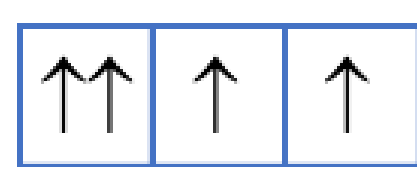
\includegraphics[height=0.9cm]{images_hoa10/page_1_img_1_48.png}} & 
\textbf{B.} \raisebox{-0.3\height}{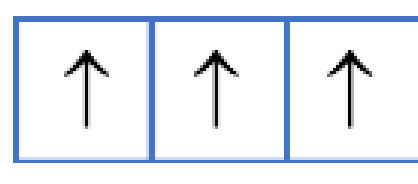
\includegraphics[height=0.9cm]{images_hoa10/page_1_img_2_50.png}} & 
\textbf{C.} \raisebox{-0.3\height}{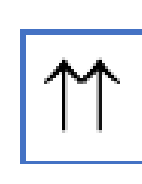
\includegraphics[height=0.9cm]{images_hoa10/page_1_img_3_52.png}} & 
\textbf{D.} \raisebox{-0.3\height}{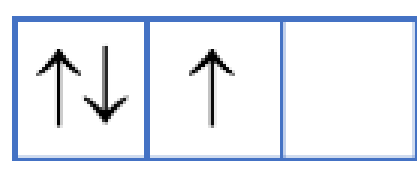
\includegraphics[height=0.9cm]{images_hoa10/page_1_img_4_54.png}} \\
\end{tabularx}
\end{center}


% CÂU 4
\textbf{Câu 4.} Lớp L có số phân lớp electron bằng
\begin{tabularx}{\textwidth}{@{}XXXX@{}}
\textbf{A.} 1. & \textbf{B.} 4. & \textbf{C.} 2. & \textbf{D.} 3. \\
\end{tabularx}


% CÂU 5
\textbf{Câu 5.} Các hạt cấu tạo nên hạt nhân của hầu hết các nguyên tử là
\begin{tabularx}{\textwidth}{@{}XX@{}}
\textbf{A.} electron và neutron. & \textbf{B.} electron, proton và neutron. \\
\textbf{C.} proton và neutron. & \textbf{D.} neutron và electron. \\
\end{tabularx}


% CÂU 6
\textbf{Câu 6.} Kí hiệu chung của mọi nguyên tử là $^{A}_{Z}\text{X}$, trong đó $A$, $Z$ và $\text{X}$ lần lượt là
\begin{enumerate}[label=\textbf{\Alph*.},leftmargin=*,itemsep=1pt,topsep=1pt]
\item số khối, số hiệu nguyên tử, kí hiệu nguyên tố.
\item số khối, kí hiệu nguyên tố, số hiệu nguyên tử.
\item số hiệu nguyên tử, kí hiệu nguyên tố, số khối.
\item số hiệu nguyên tử, số khối, kí hiệu nguyên tố.
\end{enumerate}


% CÂU 7
\textbf{Câu 7.} Nguyên tử của nguyên tố X có electron cuối cùng điền vào phân lớp $3p^1$. Nguyên tử của nguyên tố Y có electron cuối cùng điền vào phân lớp $3p^3$. Số proton của X, Y lần lượt là
\begin{tabularx}{\textwidth}{@{}XXXX@{}}
\textbf{A.} 12 và 14. & \textbf{B.} 13 và 15. & \textbf{C.} 12 và 15. & \textbf{D.} 13 và 14. \\
\end{tabularx}


% CÂU 8
\textbf{Câu 8.} Orbital s có dạng
\begin{tabularx}{\textwidth}{@{}XXXX@{}}
\textbf{A.} hình cầu. & \textbf{B.} hình số 8 nổi. & \textbf{C.} hình tròn. & \textbf{D.} hình bầu dục. \\
\end{tabularx}


% CÂU 9
\textbf{Câu 9.} Dãy nào sau đây gồm các đồng vị của cùng một nguyên tố hoá học?
\begin{enumerate}[label=\textbf{\Alph*.},leftmargin=*,itemsep=1pt,topsep=1pt]
\item $^{14}_6\text{X}$, $^{14}_7\text{Y}$, $^{14}_8\text{Z}$.
\item $^{28}_{14}\text{X}$, $^{29}_{14}\text{Y}$, $^{30}_{14}\text{Z}$.
\item $^{40}_{18}\text{X}$, $^{40}_{19}\text{Y}$, $^{40}_{20}\text{Z}$.
\item $^{19}_9\text{X}$, $^{19}_{10}\text{Y}$, $^{20}_{10}\text{Z}$.
\end{enumerate}


% CÂU 10
\textbf{Câu 10.} Lithium ($Z = 3$) là một nguyên tố có nhiều công dụng, được sử dụng trong chế tạo máy bay và trong một số loại pin nhất định. Pin Lithium-Ion (Li-Ion) đang ngày càng phổ biến, nó cung cấp năng lượng cho cuộc sống của hàng triệu người mỗi ngày thông qua các thiết bị như máy tính xách tay, điện thoại di động, xe Hybrid, xe điện,… nhờ trọng lượng nhẹ, cung cấp năng lượng cao và khả năng sạc lại. Tính chất hóa học cơ bản của lithium là
\begin{tabularx}{\textwidth}{@{}XX@{}}
\textbf{A.} khí hiếm. & \textbf{B.} vừa kim loại vừa phi kim. \\
\textbf{C.} kim loại. & \textbf{D.} phi kim. \\
\end{tabularx}


% CÂU 11
\textbf{Câu 11.} Cấu hình electron của nguyên tử P ($Z = 15$) là
\begin{tabularx}{\textwidth}{@{}XX@{}}
\textbf{A.} $1s^2 2s^2 2p^6 3s^2 3p^5$. & \textbf{B.} $1s^2 2s^2 2p^6 3s^2 3p^3$. \\
\textbf{C.} $1s^2 2s^2 2p^6 3s^1$. & \textbf{D.} $1s^2 2s^2 2p^6 3s^2 3p^2$. \\
\end{tabularx}


% CÂU 12
\textbf{Câu 12.} Số proton và số neutron có trong một nguyên tử aluminium ($^{27}_{13}\text{Al}$) lần lượt là
\begin{tabularx}{\textwidth}{@{}XXXX@{}}
\textbf{A.} 12 và 14. & \textbf{B.} 13 và 14. & \textbf{C.} 13 và 13. & \textbf{D.} 13 và 15. \\
\end{tabularx}


% =============================================================================
% PHẦN II
% =============================================================================
\vspace{6pt}
{\color{myGreen}\bfseries\large PHẦN II (2,0 ĐIỂM). Câu trắc nghiệm đúng sai.}

\textit{\small Thí sinh trả lời từ câu 1 đến câu 2. Trong mỗi ý a), b), c), d) ở mỗi câu, thí sinh chọn đúng hoặc sai.}
\vspace{3pt}

% CÂU 1 PHẦN II
\textbf{Câu 1.} Cho hình ảnh một số nguyên tố sau trong bảng tuần hoàn:
\begin{center}
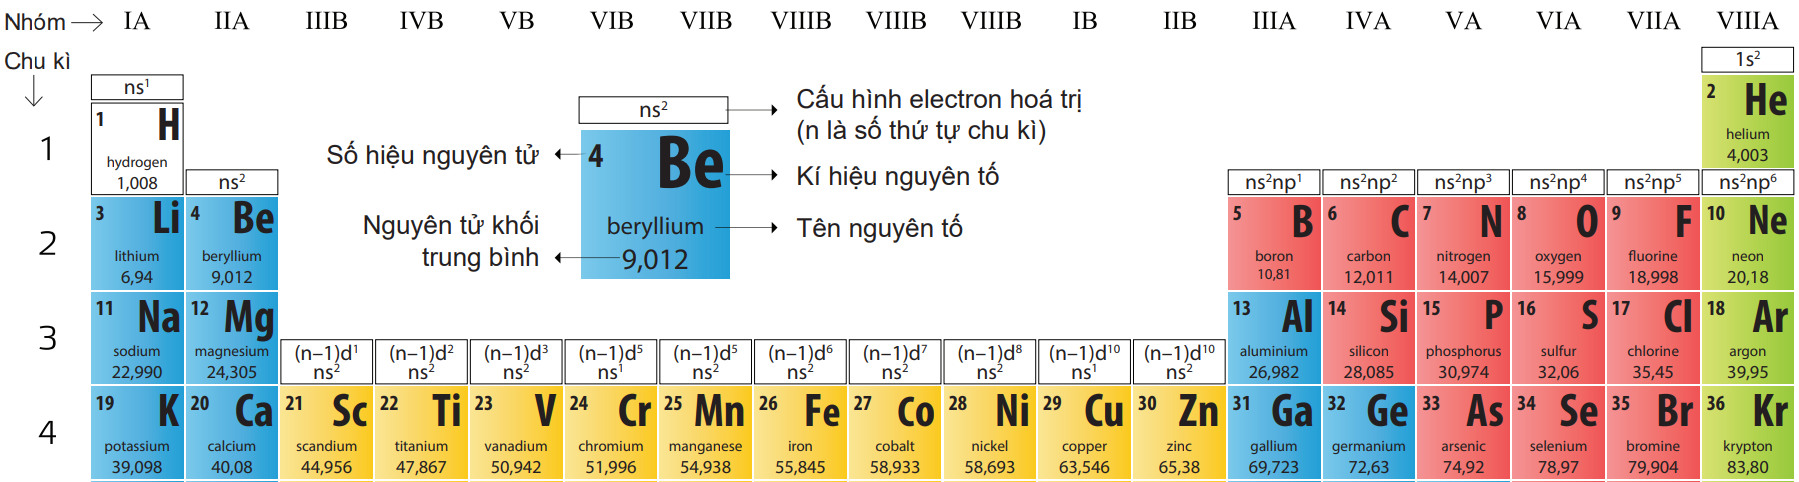
\includegraphics[width=0.98\textwidth]{images_hoa10/page_2_img_1_62.png}
\end{center}

\textit{Chọn đúng hoặc sai cho các kết luận sau:}\\
\textbf{a)} N và P có cùng số electron lớp ngoài cùng.\\

\textbf{b)} Điện tích hạt nhân của S là $+32,06$.\\

\textbf{c)} C và Li có cùng số lớp electron.\\

\textbf{d)} Có tổng 18 nguyên tố hóa học ở các chu kì nhỏ.\\


% CÂU 2 PHẦN II
\textbf{Câu 2.} Năm 1911, Rơ-đơ-pho (E. Rutherford) và các cộng sự đã dùng các hạt $\alpha$ bắn phá lá vàng mỏng và dùng màn huỳnh quang đặt sau lá vàng để theo dõi đường đi của các hạt $\alpha$. Đa số hạt $\alpha$ xuyên qua nguyên tử, một số hạt va chạm hạt nhân nguyên tử bị bật ngược trở lại hoặc bật ra hướng khác. Kết quả thí nghiệm đã rút ra các kết luận về nguyên tử như sau:

\textit{Chọn đúng hoặc sai cho các kết luận sau:}\\
\textbf{a)} Nguyên tử rỗng là nguyên nhân vì sao thể tích chất khí giảm một nửa khi tăng gấp đôi áp suất trong cùng điều kiện nhiệt độ.\\

\textbf{b)} Hạt nhân nguyên tử có kích thước rất nhỏ so với kích thước nguyên tử.\\

\textbf{c)} Hạt nhân nguyên tử tương đối đặc khít nên có một số hạt $\alpha$ bị bật ngược trở lại.\\

\textbf{d)} Nguyên tử có cấu tạo rỗng nên hạt $\alpha$ xuyên qua được.\\


% =============================================================================
% PHẦN III
% =============================================================================
\vspace{6pt}
{\color{myGreen}\bfseries\large PHẦN III (2,0 ĐIỂM). Câu trắc nghiệm trả lời ngắn.}

\textit{\small Thí sinh trả lời từ câu 1 đến câu 8.}
\vspace{3pt}

\textbf{Câu 1.} Kẽm là kim loại có ứng dụng quan trọng để bảo vệ sắt. Kí hiệu nguyên tử là $^{65}_{30}\text{Zn}$. Tính tổng số hạt proton, neutron và electron trong nguyên tử Zn.\\
\textit{Trả lời:} \dotfill\par\vspace{2pt}

\textbf{Câu 2.} Potassium (K) là kim loại có tính khử mạnh, phân mức năng lượng cao nhất là $4s^1$. Tổng số electron lớp thứ 3 của K bằng bao nhiêu?\\
\textit{Trả lời:} \dotfill\par\vspace{2pt}

\textbf{Câu 3.} Nguyên tố X thuộc chu kì 2. Vậy X có bao nhiêu lớp electron?\\
\textit{Trả lời:} \dotfill\par\vspace{2pt}

\textbf{Câu 4.} Trong phân tử $\text{MX}_2$ có tổng số hạt là 164, trong phân tử số hạt mang điện nhiều hơn số hạt không mang điện là 52 hạt. Số khối của nguyên tử M lớn hơn số khối của nguyên tử X là 5. Tổng số hạt trong 1 nguyên tử M nhiều hơn trong 1 nguyên tử X là 8 hạt. Tính số khối của M.\\
\textit{Trả lời:} \dotfill\par\vspace{2pt}

\textbf{Câu 5.} Carbon là phi kim có ứng dụng phổ biến trong đời sống như nhiên liệu, làm mặt nạ phòng độc, trang sức. Nguyên tử carbon có hai đồng vị bền: $^{12}_6\text{C}$ và $^{13}_6\text{C}$. Nguyên tử khối trung bình của carbon là 12,01. Thành phần phần trăm số nguyên tử của đồng vị $^{13}_6\text{C}$ là bao nhiêu?\\
\textit{Trả lời:} \dotfill\par\vspace{2pt}

\textbf{Câu 6.} Kim loại X có ứng dụng lớn trong đời sống như làm vật liệu xây dựng, xoong, chảo. Cho ion $\text{XO}_2^-$ với O là nguyên tử oxygen (biết O có 8 proton). Tổng số electron trong ion trên bằng 30. Tổng số hạt mang điện trong nguyên tử X là bao nhiêu?\\
\textit{Trả lời:} \dotfill\par\vspace{2pt}

\textbf{Câu 7.} Nguyên tử X có điện tích hạt nhân bằng $+9$. Số electron độc thân của X ở trạng thái cơ bản là bao nhiêu?\\
\textit{Trả lời:} \dotfill\par\vspace{2pt}

\textbf{Câu 8.} Nguyên tử Y có phân lớp năng lượng cao nhất là $3p^3$. Tổng số electron của Y là bao nhiêu?\\
\textit{Trả lời:} \dotfill\par\vspace{2pt}

% =============================================================================
% PHẦN IV
% =============================================================================
\vspace{6pt}
{\color{myGreen}\bfseries\large PHẦN IV (3,0 ĐIỂM). Tự luận.}

\textit{\small Thí sinh làm từ câu 1 đến câu 3 ra giấy làm bài thi tự luận.}
\vspace{3pt}

\textbf{Câu 1 (1,0 điểm).} Cho nguyên tố hydrogen có ba đồng vị $^1_1\text{H}, ^2_1\text{H}, ^3_1\text{H}$.\\
\textbf{a)} \textit{(0,25 điểm)} Xác định số proton, neutron và electron của đồng vị $^1_1\text{H}$.\\

\textbf{b)} \textit{(0,25 điểm)} Dựa vào đâu người ta ghi khối lượng nguyên tố hydrogen vào trong bảng tuần hoàn?\\

\textbf{c)} \textit{(0,25 điểm)} Phân tử nước có công thức là $\text{H}_2\text{O}$. Cho biết nguyên tố oxygen có 3 đồng vị bền $^{16}_8\text{O}, ^{17}_8\text{O}, ^{18}_8\text{O}$. Em hãy cho biết phân tử nước có khối lượng nặng nhất là bao nhiêu amu (chấp nhận khối lượng nguyên tử bằng số khối)?\\

\textbf{d)} \textit{(0,25 điểm)} Có bao nhiêu phân tử nước được hình thành từ đồng vị $^{16}_8\text{O}$?\\
\noindent\dotfill\\
\noindent\dotfill\\
\noindent\dotfill\par\vspace{3pt}


\textbf{Câu 2 (1,0 điểm).} Sodium (Na) là nguyên tố quan trọng, có nhiều trong nước biển ở dạng muối NaCl. Na có số hiệu nguyên tử là 11.\\
\textbf{a)} \textit{(0,25 điểm)} Xác định số electron của Na.\\

\textbf{b)} \textit{(0,25 điểm)} Viết cấu hình electron nguyên tử của Na.\\

\textbf{c)} \textit{(0,25 điểm)} Na là kim loại, phi kim hay khí hiếm?\\

\textbf{d)} \textit{(0,25 điểm)} Cho nguyên tử khối trung bình của Na và Cl lần lượt là 22,99 và 35,5. Na có hai đồng vị $^{23}_{11}\text{Na}, ^{22}_{11}\text{Na}$. Tính phần trăm khối lượng của $^{22}_{11}\text{Na}$ trong phân tử NaCl.\\
\noindent\dotfill\\
\noindent\dotfill\\
\noindent\dotfill\par\vspace{3pt}


\textbf{Câu 3 (1,0 điểm).} Cho nguyên tố X ở chu kì 2 và có 4 electron lớp ngoài cùng.\\
\textbf{a)} \textit{(0,25 điểm)} X có bao nhiêu lớp electron?\\

\textbf{b)} \textit{(0,25 điểm)} X ở nhóm nào trong bảng hệ thống tuần hoàn?\\

\textbf{c)} \textit{(0,25 điểm)} Nguyên tố Y ở cùng chu kì với X và có nhiều hơn X hai đơn vị điện tích hạt nhân. Xác định số electron của Y.\\

\textbf{d)} \textit{(0,25 điểm)} Hợp chất của X và Y có công thức $\text{XY}_2$. Tính tổng số proton trong phân tử $\text{XY}_2$.\\
\noindent\dotfill\\
\noindent\dotfill\\
\noindent\dotfill\par\vspace{3pt}


\begin{center}
\textbf{--- HẾT ---}
\end{center}
\end{document}